% GNUPLOT: LaTeX picture with Postscript
\begingroup
  \makeatletter
  \providecommand\color[2][]{%
    \GenericError{(gnuplot) \space\space\space\@spaces}{%
      Package color not loaded in conjunction with
      terminal option `colourtext'%
    }{See the gnuplot documentation for explanation.%
    }{Either use 'blacktext' in gnuplot or load the package
      color.sty in LaTeX.}%
    \renewcommand\color[2][]{}%
  }%
  \providecommand\includegraphics[2][]{%
    \GenericError{(gnuplot) \space\space\space\@spaces}{%
      Package graphicx or graphics not loaded%
    }{See the gnuplot documentation for explanation.%
    }{The gnuplot epslatex terminal needs graphicx.sty or graphics.sty.}%
    \renewcommand\includegraphics[2][]{}%
  }%
  \providecommand\rotatebox[2]{#2}%
  \@ifundefined{ifGPcolor}{%
    \newif\ifGPcolor
    \GPcolortrue
  }{}%
  \@ifundefined{ifGPblacktext}{%
    \newif\ifGPblacktext
    \GPblacktexttrue
  }{}%
  % define a \g@addto@macro without @ in the name:
  \let\gplgaddtomacro\g@addto@macro
  % define empty templates for all commands taking text:
  \gdef\gplbacktext{}%
  \gdef\gplfronttext{}%
  \makeatother
  \ifGPblacktext
    % no textcolor at all
    \def\colorrgb#1{}%
    \def\colorgray#1{}%
  \else
    % gray or color?
    \ifGPcolor
      \def\colorrgb#1{\color[rgb]{#1}}%
      \def\colorgray#1{\color[gray]{#1}}%
      \expandafter\def\csname LTw\endcsname{\color{white}}%
      \expandafter\def\csname LTb\endcsname{\color{black}}%
      \expandafter\def\csname LTa\endcsname{\color{black}}%
      \expandafter\def\csname LT0\endcsname{\color[rgb]{1,0,0}}%
      \expandafter\def\csname LT1\endcsname{\color[rgb]{0,1,0}}%
      \expandafter\def\csname LT2\endcsname{\color[rgb]{0,0,1}}%
      \expandafter\def\csname LT3\endcsname{\color[rgb]{1,0,1}}%
      \expandafter\def\csname LT4\endcsname{\color[rgb]{0,1,1}}%
      \expandafter\def\csname LT5\endcsname{\color[rgb]{1,1,0}}%
      \expandafter\def\csname LT6\endcsname{\color[rgb]{0,0,0}}%
      \expandafter\def\csname LT7\endcsname{\color[rgb]{1,0.3,0}}%
      \expandafter\def\csname LT8\endcsname{\color[rgb]{0.5,0.5,0.5}}%
    \else
      % gray
      \def\colorrgb#1{\color{black}}%
      \def\colorgray#1{\color[gray]{#1}}%
      \expandafter\def\csname LTw\endcsname{\color{white}}%
      \expandafter\def\csname LTb\endcsname{\color{black}}%
      \expandafter\def\csname LTa\endcsname{\color{black}}%
      \expandafter\def\csname LT0\endcsname{\color{black}}%
      \expandafter\def\csname LT1\endcsname{\color{black}}%
      \expandafter\def\csname LT2\endcsname{\color{black}}%
      \expandafter\def\csname LT3\endcsname{\color{black}}%
      \expandafter\def\csname LT4\endcsname{\color{black}}%
      \expandafter\def\csname LT5\endcsname{\color{black}}%
      \expandafter\def\csname LT6\endcsname{\color{black}}%
      \expandafter\def\csname LT7\endcsname{\color{black}}%
      \expandafter\def\csname LT8\endcsname{\color{black}}%
    \fi
  \fi
  \setlength{\unitlength}{0.0500bp}%
  \begin{picture}(6046.00,3325.00)%
    \gplgaddtomacro\gplbacktext{%
      \csname LTb\endcsname%
      \put(1781,1087){\makebox(0,0)[r]{\strut{}\sf 10}}%
      \csname LTb\endcsname%
      \put(1781,1581){\makebox(0,0)[r]{\strut{}\sf 20}}%
      \csname LTb\endcsname%
      \put(1781,2074){\makebox(0,0)[r]{\strut{}\sf 30}}%
      \csname LTb\endcsname%
      \put(1781,2568){\makebox(0,0)[r]{\strut{}\sf 40}}%
      \csname LTb\endcsname%
      \put(1781,3061){\makebox(0,0)[r]{\strut{}\sf 50}}%
      \csname LTb\endcsname%
      \put(1781,1087){\makebox(0,0)[r]{\strut{}}}%
      \csname LTb\endcsname%
      \put(1781,1581){\makebox(0,0)[r]{\strut{}}}%
      \csname LTb\endcsname%
      \put(1781,2074){\makebox(0,0)[r]{\strut{}}}%
      \csname LTb\endcsname%
      \put(1781,2568){\makebox(0,0)[r]{\strut{}}}%
      \csname LTb\endcsname%
      \put(1781,3061){\makebox(0,0)[r]{\strut{}}}%
      \csname LTb\endcsname%
      \put(1913,385){\makebox(0,0){\strut{}\sf 0}}%
      \csname LTb\endcsname%
      \put(2282,385){\makebox(0,0){\strut{}\sf 1}}%
      \csname LTb\endcsname%
      \put(2650,385){\makebox(0,0){\strut{}\sf 2}}%
      \csname LTb\endcsname%
      \put(3019,385){\makebox(0,0){\strut{}\sf 3}}%
      \csname LTb\endcsname%
      \put(3388,385){\makebox(0,0){\strut{}\sf 4}}%
      \csname LTb\endcsname%
      \put(3756,385){\makebox(0,0){\strut{}\sf 5}}%
      \csname LTb\endcsname%
      \put(4125,385){\makebox(0,0){\strut{}\sf 6}}%
      \csname LTb\endcsname%
      \put(4494,385){\makebox(0,0){\strut{}\sf 7}}%
      \csname LTb\endcsname%
      \put(4862,385){\makebox(0,0){\strut{}\sf 8}}%
      \csname LTb\endcsname%
      \put(5231,385){\makebox(0,0){\strut{}\sf 9}}%
      \put(5363,697){\makebox(0,0)[l]{\strut{}\sf 1}}%
      \put(5363,1302){\makebox(0,0)[l]{\strut{}\sf 2}}%
      \put(5363,1907){\makebox(0,0)[l]{\strut{}\sf 4}}%
      \put(5363,2512){\makebox(0,0)[l]{\strut{}\sf 8}}%
      \put(5363,2866){\makebox(0,0)[l]{\strut{}\sf 12}}%
      \put(1275,1833){\rotatebox{90}{\makebox(0,0){\strut{}\sf Temperature  ($\mu$K)}}}%
      \put(5789,1833){\rotatebox{90}{\makebox(0,0){\strut{}\sf Number/ $\mathsf{10^{5}}$}}}%
      \put(3572,154){\makebox(0,0){\strut{}\sf Evaporation time (s)}}%
    }%
    \gplgaddtomacro\gplfronttext{%
      \csname LTb\endcsname%
      \put(4696,2831){\makebox(0,0)[r]{\strut{}$\sf U(t)/10$}}%
      \csname LTb\endcsname%
      \put(4696,2568){\makebox(0,0)[r]{\strut{}$\sf N(t)$}}%
      \csname LTb\endcsname%
      \put(4696,2305){\makebox(0,0)[r]{\strut{}$\sf T(t)$}}%
    }%
    \gplbacktext
    \put(525,0){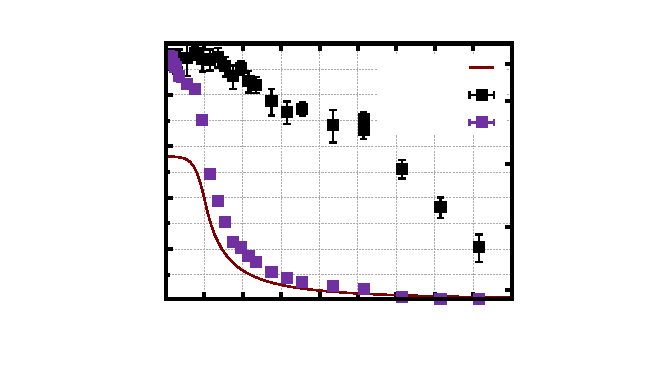
\includegraphics{evap}}%
    \gplfronttext
  \end{picture}%
\endgroup
